\section{Bakti QIlan Mufid (1174083)}
\subsection{Buku}
Rp.100.000(Lunas)
\subsection{Data Geospasial}
\begin{itemize}
\item Geospasial data atau juga bisa disebut dengan Spatial Data atau GIS (Geospatial Information System data) adalah tentan g aspek fisik dan adminsitratif dari sebuah objek geografis. Aspek fisik ini mencakup pula bentuk anthropogenic dan bentuk alam baik yang terdiri dari permukaan maupun dibawah permukaan bumi. Bentuk anthropogenic mengandung didalamnya fenomena budaya seperti jalan, rel kereta api, bangunan, jembatan, dan sebagainya. Bentuk alam tentusaja seperti sungai, danau, pantai, dataran tinggi, dan sebagainya. Sedangkan aspek administratif adalah pembagian atau pembatasan sosio-kultular yang dibuat oleh suatu organisasi atau badan untuk keperluan pengaturan dan pemakaian sumberdaya alam. Termasuk dalam aspek administratif ini adalah batas negara, pembagian wilayah administrasi, zona, kode pos, batas kepemilikan tanah, dan sebagainya.

\item SIG mulai dikenal pada awal 1980-an. Sejalan dengan berkembangnya perangkat komputer, baik perangkat lunak maupun perangkat keras, SIG berkembang sangat pesat pada era 1990-an.

\item Secara harafiah, SIG dapat diartikan sebagai : \textit{”suatu komponen yang terdiri dari perangkat keras, perangkat lunak, data geografis dan sumberdaya manusia yang bekerja bersama secara efektif untuk menangkap, menyimpan, memperbaiki, memperbaharui, mengelola, memanipulasi, mengintegrasikan, menganalisa, dan menampilkan data dalam suatu informasi berbasis geografis”} 

\item Secara umum terdapat dua metode untuk menampilkan fitur geografis ke dalam GIS atau Sistem Informasi Geospasial:
	\begin{enumerate}
	\item Data Raster  (raster data structure)Terdiri dari serangkaian sel atau pixels yang biasa dipakai untuk menggambarkan data gambar sebagai data yang berkesinambungan. Dalam struktur data yang demikian, ada unsur resolusi sebagai ukuran dari dimensi fitur geografis yang terwakili dalam bentuk pixel. Biasanya data raster ini dipakai untuk citra satelit, ortografi digital, model elevasi digital (digital elevation models, DEM), peta digital, dan sebagainya.
	\begin{figure}[H]
	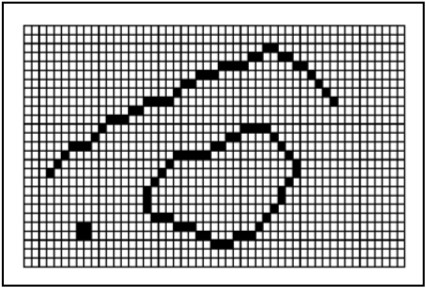
\includegraphics[width=4cm]{figures/Tugas1/1174083/Raster.jpg}
	\centering
	\caption{Data Raster}
	\end{figure}
	\item Data Vektor (vector data structure)Terdiri dari sebuah gambaran titik geografis, baik yang berupa tanda titik, garis, maupun poligon. Model grafik vektor ini menampilkan secara terpisah fitur geografis seperti batas administratif, jalan, bangunan, dan sungai. Sebuah objek grafis biasanya dikaitkan dengan informasi yang mengandung penjelasan tentang atribut objek itu, dan informasi ini bisa saja disimpan di dalam berkas spreadsheets atau pangkalan data terpisah.
	\begin{figure}[H]
	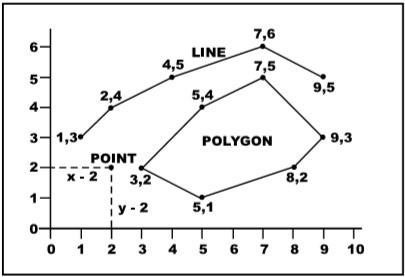
\includegraphics[width=4cm]{figures/Tugas1/1174083/vektor.jpg}
	\centering
	\caption{Data Vektor}
	\end{figure}
	\end{enumerate}
\end{itemize}

\subsection{Link}
http://bit.ly/baktiGEO
\subsection{Plagiarism}
	\begin{figure}[H]
	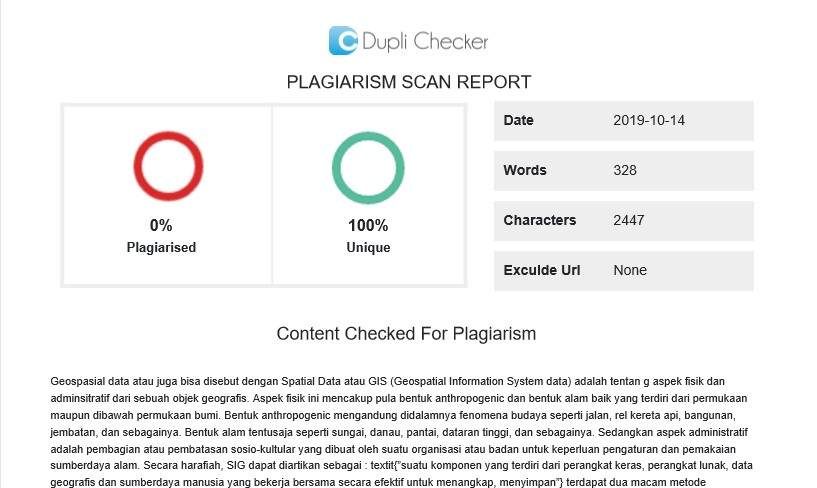
\includegraphics[width=4cm]{figures/Tugas1/1174083/plagiarsm.jpg}
	\centering
	\caption{check plagiarsm}
	\end{figure}

\subsection{Cara Penggunaan}
\subsubsection{Gambar}

\hfill\break

Contoh Gambar
\begin{figure}[H]
	
\includegraphics[width=4cm]{figures/himatif.png}
	\centering
	\caption{Contoh gambar.}
\end{figure}

\subsubsection{List}
\begin{enumerate}
	\item Satu
	\item Dua
\end{enumerate}

\begin{itemize}
	\item Satu
	\item Dua
\end{itemize}

